

\begin{center}
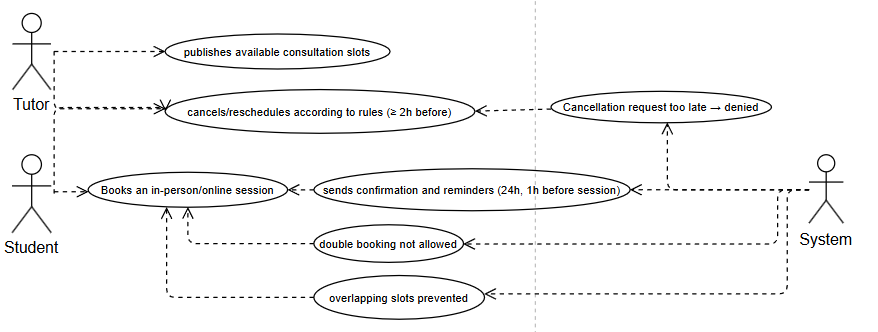
\includegraphics[width=0.9\linewidth]{images/UC-03.png}
\end{center}

\begin{center}
\textbf{Figure 4:}  Session Scheduling Management
\end{center}

\begin{table}[h!]
\centering
\begin{tabular}{|p{3cm}|p{11cm}|}
\hline
\textbf{Use-case ID} & UC-03 \\
\hline
\textbf{Use-case name} & Session Scheduling Management \\
\hline
\textbf{Use-case overview} & This use case describes the end-to-end process of session scheduling between a student and a tutor, including slot publication, booking, cancellation, rescheduling, and automatic notifications. \\
\hline
\textbf{Actors} & Student, Tutor, System \\
\hline
\textbf{Preconditions} & 
1. Student is matched with a tutor. \newline
2. Tutor has published available slots. \newline
3. System is operational and connected to the scheduling database. \\
\hline
\textbf{Trigger} & 
1. Tutor publishes or edits availability slots. \newline
2. Student attempts to book a session. \newline
3. Student or tutor submits a cancellation or rescheduling request. \\
\hline
\textbf{Steps} & 
1. Tutor publishes available consultation slots. \newline
2. System prevents overlapping slots. \newline
3. Student views available slots. \newline
4. If a slot is suitable, student books a session. \newline
5. System prevents double-booking and stores session details. \newline
6. System confirms the booking and sends notifications. \newline
7. Before the session, the system sends reminders (24h and 1h before). \newline
8. Student or tutor may request cancellation or rescheduling at least 2 hours before the session. \newline
9. System validates the request: if valid, cancels/reschedules and sends notifications; otherwise denies the request. \\
\hline
\textbf{Postconditions} & 
1. Session is successfully scheduled, rescheduled, or cancelled according to rules. \newline
2. Notifications and reminders are delivered to all relevant parties. \\
\hline
\textbf{Exception Flow} & 
1. Overlapping slots → publishing is denied. \newline
2. Double-booking attempt → booking is denied. \newline
3. No suitable slot → student is prompted to wait or check later. \newline
4. Late cancellation → request is denied. \\
\hline
\end{tabular}
\caption{Use Case UC-03: Session Scheduling Management}
\end{table}
